\section{Methods} \label{sec:methods}

In the following, we define the terminology used in the study, the process and criteria for selecting a set of \acp{ide} for the study, the definition of a set of novel visual \ac{ide} interface features, and the process of evaluation taken for each \ac{ide}.

\subsection{Terminology \jmr{Just added this}} \label{subsec:terminology}
The \emph{workspace} of an \ac{ide} is sometimes referred to as a
\emph{canvas} and is an area within the \ac{ide} interface with which the
operator directly interacts to create and store content. Generally the
workspace does not contain a listing of available tools. An active
workspace is highlighted in \Fig{fig:workspace}. The \emph{supported
language} of an \ac{ide} is the visual language the \ac{ide} allows its
user to work in. The \ac{ide} includes features and tools to support
development within this language.  \emph{Elements} within the language are
syntactic units or lexemes represented visually within the \ac{ide}
workspace. Similarly, \emph{relations} or \emph{connections} are syntactic
relationships between elements represented visually within the workspace.
\cite{costagliola2002} See \Fig{fig:elements} for a visual representation
of elements and relations.

\begin{figure}[!t]
\centering
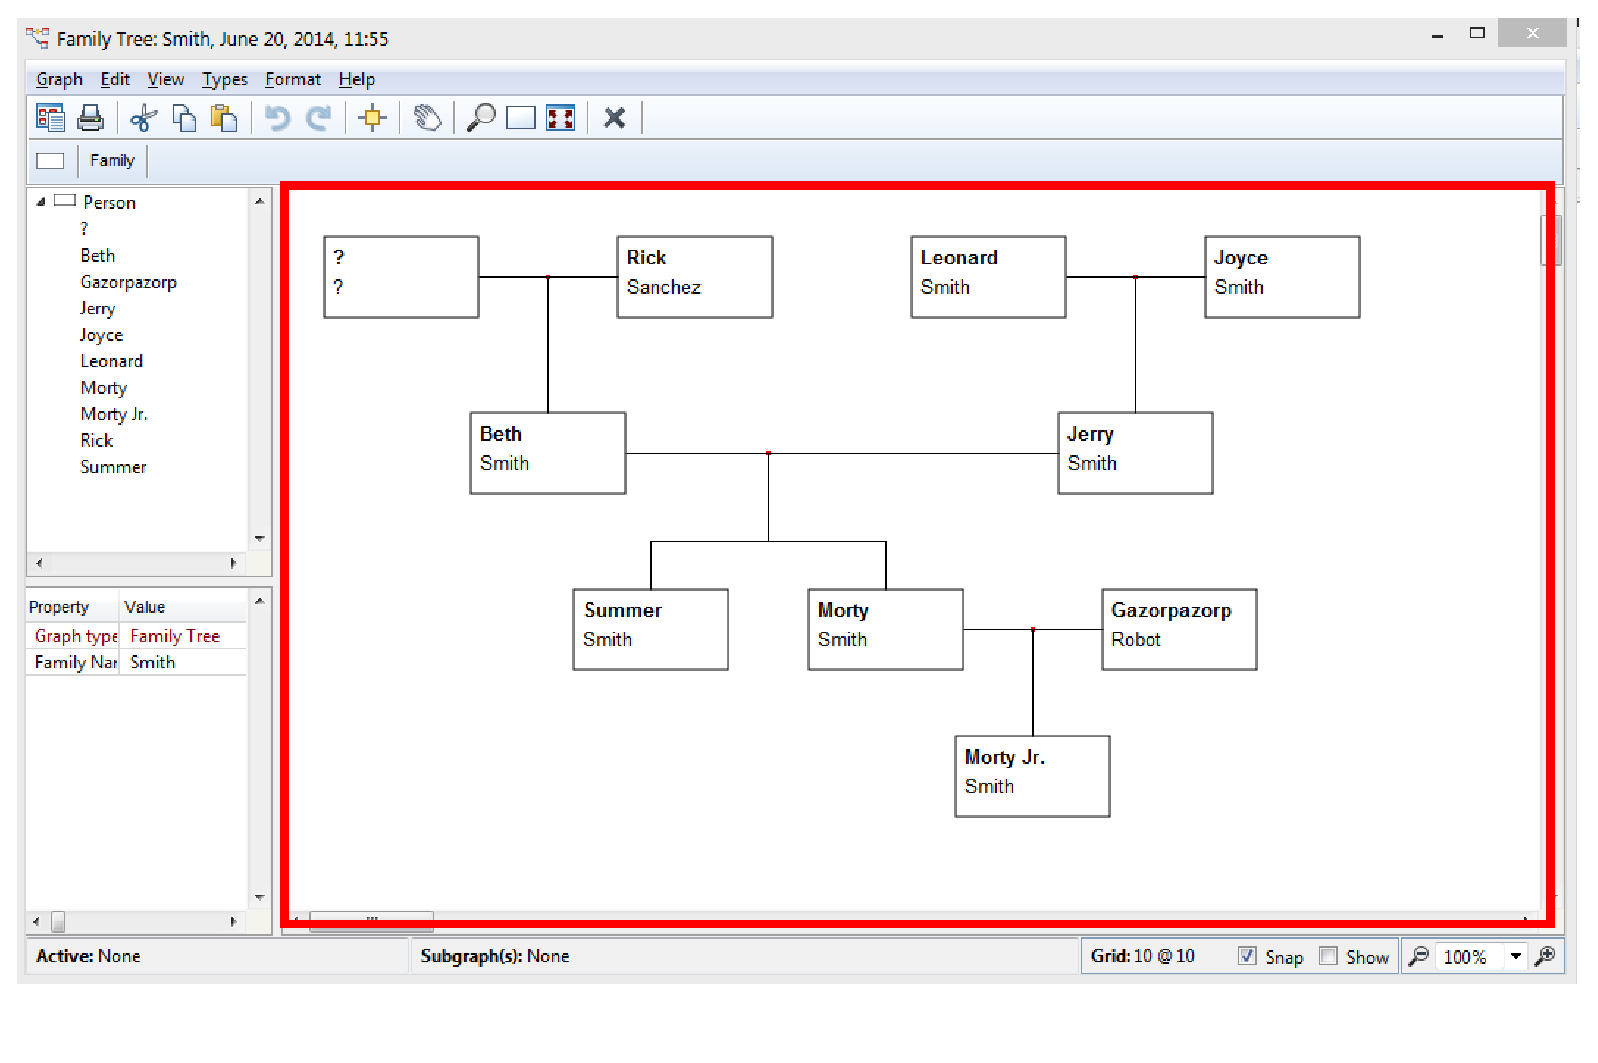
\includegraphics[width=3in]{images/workspace}
\caption{An ide workspace highlighted in red}
\label{fig:workspace}
\end{figure}

\begin{figure}[!t]
\centering

\includegraphics[width=1.5in]{images/element}
\caption{Two elements connected by a relationship}
\label{fig:elements}
\end{figure}


\subsection{\acs{ide} Selection} \label{subsec:ideselection}

We decided to select \acp{ide} based on their support for a visual language
as the primary language of development.  A subsidiary criteria for
selection included popularity of the \ac{ide} within its domain as well as
representation from a variety of development domains.  Thus this survey
considers \acp{ide} from eight different domains: 3D modeling, animation,
modeling, music, prototyping, simulation, software development (\eg
education, mobile development, etc.), and business workflow.


\subsection{Feature Definition} \label{subsec:featuredefinition}

The following enumerates a unique set of features based on existing literature, and the emergence of similarities and differences between the \acp{ide} considered.
Features are categorized under the following five headings.


\subsubsection{Audience Features} \label{subsubsec:audience}

The audience of an \ac{ide} refers generally to the target populations for which
the \ac{ide} is intended.


\paragraph{Domain}
The domain of an \ac{ide} refers to the domain or field of
knowledge under which the interface falls.
%That is, the field or fields for which the interface is primarily used, if any.
This is a nominal variable where example values might include \texttt{General}, \texttt{Modeling}, \texttt{Software}, etc.
The latter \texttt{General} indicates that the \ac{ide} is of general purpose and can be applied within any number of different fields to the same extent.


\paragraph{Skill Level}
The skill level of an \ac{ide} describes what level of domain expertise is expected of users for using it.
This is a nominal variable where possible values are \texttt{Novice}, \texttt{Intermediate}, \texttt{Expert}, and \texttt{General}.
The latter indicates that the \ac{ide} offers a powerful set of advanced features while maintaining components that emphasize accessibility and ease of use.


\subsubsection{Chrome Features} \label{subsubsec:chrome}

The chrome of an \ac{ide} is the total set of all \acf{gui} components
external to the workspace. This includes every tool, menu, button, or other
user interface component not contained within the workspace area.


\paragraph{General Operations}
Many \acp{ide} provide support for a specific subset of common operations.
\citeauthor{murphy2006}~\cite{murphy2006} define a list of the top 10 \ac{ide} features most frequently utilized by developers.
We reproduced it here as a set of Boolean sub-variables that indicates whether the \ac{ide} in question supports the use of that particular operation.
We report the sum of the \texttt{true} values.
The operations are: \emph{delete} a syntactic element in the workspace,
\emph{save} to export a model to storage media,
\emph{cut}/\emph{copy}/\emph{paste} an existing syntactic element in the workspace,
\emph{content assist} that provides suggestions or completion for elements,
 to place an existing syntactic element from the workspace into paste buffer,
\emph{undo} the user's most recent action,
\emph{refresh} to load contents of workspace and interface dashboard elements from storage media and update display if necessary.
\emph{show view} opens and displays a new tool in the interface,
and
\emph{next word} moves active selection to the next element according to some natural ordering, for example as a result of searching.


\paragraph{Context Sensitive Tools}
Any interface component which changes visibly or is generated anew
depending on the context of selected elements within the workspace is
context sensitive, \eg a popup context menu that appears when an element is
clicked which provides tools or information about the clicked element.
This Boolean variable indicates whether context sensitive tools are
supported.
\es{example.} \jmr{addressed}


\paragraph{Degree of Interface Visual Richness}
This describes the extent to which an \ac{ide} utilizes visual variables to increase the visual discrimination of tools it offers.
This compound variable is composed of eight sub-variables, each being a Boolean measure determining whether or not the described visual variable is utilized in the interface to distinguish between available tools in the \ac{ide}.
We report the sum of the \texttt{true} values.
The variables include:
\emph{icons}~\cite{costagliola2002,moody2009} as images contained in a border of a standard size and shape,
\emph{shapes}~\cite{moody2009},
tool \emph{size}~\cite{moody2009},
\emph{color}~\cite{moody2009},
\emph{text} or typographic variation~\cite{moody2009},
\emph{texture}~\cite{moody2009} as shading or shadows,
\emph{brightness} of a color (\ie its perceived luminosity)~\cite{moody2009},
and
\emph{organizational coherence}~\cite{constantine1996} to determine if components with related purpose are visually grouped together in the interface.


\paragraph{Multiplicity of Perspectives}
A perspective is defined as a visual configuration of tools in the \ac{gui}
for the purpose of accomplishing a distinct task as part of a distinct
process, \eg debugging, file browsing, manipulation of element details.
Some \acp{ide}, \eg MST Workshop, even support multiple languages or
domains through the use of perspectives by offering entirely different
feature sets. This metric measures the number of available predefined
interface perspectives available to the user, with values greater than
zero.
\es{example.}\jmr{addressed}


\paragraph{Object Properties Window}
This is an interface component that displays the properties of an element
in the workspace, typically to view and modify properties of model
elements.  For example, the \ac{ide} \ac{grc} allows elements to take
user-defined values for various properties (\eg frequency, amplitude).
These properties can be manipulated when the user explicitly requests the
properties dialog window for that element.
\es{example.}\jmr{addressed}
This is a nominal variable whose values are:
\texttt{None} if no object properties window is available,
\texttt{Omnipresent} if such window is always present, allowing contents to update contextually,
and \texttt{Manual} if such window requires user interaction to bring forward.


\paragraph{Searchable Toolspace}
This is a Boolean variable that indicates whether the total set of
available tools, components, or actions offered by the \ac{ide} can be
searched through by name or keyword, \eg \cameleon~which provides the user
a search box to navigate its library of predefined available elements.
\es{example.}\jmr{addressed}


\paragraph{Toolbar Styles}
These refer to the set of \ac{gui} component idioms employed by the \ac{ide}~\cite{galitz2007}.
This nominal variable can take combinations of multiple values, such as:
\texttt{Icons}, \texttt{Menus}, \texttt{Ribbons}, \texttt{Trees}.


\paragraph{Visual Clutter}
The clutter of an interface is the number and organization of tools available on the screen versus the amount of workspace provided by the \ac{ide}\es{cite?}.
If the \ac{ide} offers no method for tool organization or if there is an immense amount of tools visible at once, then the \ac{ide} is likely to be visually cluttered.
\es{example.}
Visual clutter is a nominal variable and takes the values \texttt{Low}, \texttt{Medium}, or \texttt{High}.
\Sect{subsec:ideevaluation} includes details on the proper evaluation of this qualitative feature.


\subsubsection{Human Interface Features} \label{subsubsec:humaninterface}

The human interface features of an \ac{ide} include aspects of the software
interface that affect how the user interacts with the \ac{ide}, either
mechanically (\eg through physical devices and media) or mentally (\eg the
mental load required of the user to operate the \ac{ide}).


\paragraph{Essential Efficiency}
The essential efficiency of an \ac{ide} measures the level to which the system automates tasks for the user.
It is calculated as the ratio of the number of steps in a concrete use case $C$ to the number of steps in the essential use case $E$ as depicted in \Eq{eq:eefficiency}.
A concrete use case describes the steps in the specific \ac{ide} to perform the same tasks as in an essential use case.
This metric, unlike those for automation put forth in~\cite{wei1998}, does not require user experience reports and can be measured through simple use case analysis.
\Sect{subsec:ideevaluation} gives more details on the essential use cases considered.
%
\begin{align}\label{eq:eefficiency}
  1 - \frac{C}{E}
\end{align}


\paragraph{Interface Efficiency}
The interface efficiency of an \ac{ide} is a concept related to the productivity of an interface.
It measures the number of physical actions (including keystrokes, mouse clicks, and fine mouse movements) $A$ required of the user to complete a task compared against the number of abstract steps in the essential use case, as depicted in \Eq{eq:iefficiency}.
%
\begin{align}\label{eq:iefficiency}
  1 - \frac{A}{E}
\end{align}
%
This metric is different from the Essential Efficiency proposed in~\cite{constantine1996} because it studies physical user actions instead of concrete task steps.
Also note that this variable can take negative values, indicating that the number of physical actions required to complete an essential use case exceeds the number of abstract steps in the use case.


\paragraph{Keyboard Use}
This refers to the extent to which an \ac{ide} utilizes the use of a keyboard.
This can range from a complete absence of any keyboard actions to providing
certain actions which only a keyboard can perform. Keybindings (optional or
required) are a common way to provide keyboard interactivity.
\es{example.}\jmr{addressed}

This nominal variable can take the values:
\texttt{None} when no keyboard use is supported,
\texttt{Simple} when the keyboard is used only for typing annotations, properties, or comments,
\texttt{Optional} when the option to use the keyboard to execute some actions is present, but these actions can also be completed using a mouse,
and \texttt{Required} when there are actions that can only be completed through the use of the keyboard, no mouse equivalent is available.


\paragraph{Mode of Element Creation}
This describes the process through which the user creates elements in the \ac{ide}.
The \emph{Drag n Drop} process refers to a single mouse press event followed by a dragging motion of the mouse and completed when the mouse button is released.
\es{example.}
The \emph{Point n Click} process utilizes a single mouse click to indicate a selection and followed with subsequent mouse clicks elsewhere to define placement.
\es{example.}
This nominal variable can take one of four possible values created by
combining \texttt{Drag n Drop} or \texttt{Point n Click} with the
multiplicity of the action: either \texttt{(1:1)} or \texttt{(1:n)}. The
former multiplicity indicates that a single element is created for each
action, while the latter indicates that multiple can be created after the
action.


\paragraph{Tertiary Interface Devices}
This nominal variable describes any
third party human interface devices which can be used to interact with the
\ac{ide}. This could include audio devices such as MIDI keyboards or
microphones, mobile integration, etc. Variable values are the type of
tertiary devices allowed for the \ac{ide}. AudioMulch and Max, for example,
allow for the integration of microphones as data input devices. AppInventor
supports exporting to mobile devices.
\es{example.}\jmr{addressed}


\subsubsection{Integration Features} \label{subsubsec:integration}

Integration is the manner with which the \ac{ide} integrates with the visual
language it supports. This includes any visual representation of language
syntax or semantics, as well as any tools to assist the user with
understanding the supported language.


\paragraph{Allowed Relations Indicated}
This refers to an \ac{ide}'s ability to
emphasize possible syntactically correct connection points. This is often
demonstrated with either the highlighting of allowed relations or the
dimming of impossible relations, \eg \cameleon~which color codes available
connection endpoints when the operator begins creating a connection.
\es{example.}\jmr{addressed}
Boolean values indicate whether the \ac{ide} supports this feature or not.


\paragraph{Output Generation Style}
This nominal variable describes the
mode with which the \ac{ide} renders and displays output to the user. It is a
dual axis nominal variable, measuring whether output is direct or indirect
as well as live or caused by a trigger. \texttt{Direct/indirect} describes
whether the user directly modifies output or acts via a layer of
abstraction (\eg via a model as in Grasshopper, or directly as in Blender).
\es{example.}\jmr{addressed}
\texttt{Live/trigger} describes whether output is generated and displayed
live or after some event triggered by the user, \eg a compilation or build
request.
\es{example.}\jmr{addressed}


\paragraph{Syntax Enforcement}
The level of syntax enforcement of an \ac{ide} describes the mode with
which the \ac{ide} enforces its supported language's syntax requirements,
if at all.
\es{example.}
The nominal value \texttt{Explicit}
indicates that the \ac{ide} explicitly enforces syntax requirements by
indicating to the user the presence of any syntax errors. \texttt{Implicit}
enforcement indicates that the \ac{ide} does not allow syntactically illegal
operations to occur in the first place by means of some structural
mechanism. The value \texttt{None} indicates that the \ac{ide} does not support
syntax enforcement and the user is required to review their models' syntax
manually.


\subsubsection{Language Syntax Features} \label{subsubsec:languagesyntax}

Language syntax variables describe properties of the supported visual
language syntax. While not strictly components of the \ac{ide}, they are
intimately tied to the overall style of the \ac{ide} and thus included in this
study.


\paragraph{Complexity Management}
Any characteristics or features of the
visual language that serve to reduce the complexity of that language.
Reducing complexity refers specifically to decreasing the level of
\emph{diagrammatic complexity} while maintaining information transfer to
the user~\cite{moody2009}. This can be implemented variously, \eg
modularization of large projects into files or hierarchical abstraction
into levels of detail.
\es{example.}\jmr{addressed?}
This nominal variable can take one of three possible values.
\texttt{Modularization} indicates that large systems within the language
are divided into smaller subsystems to reduce complexity~\cite{moody2009}.
\texttt{Hierarchy} indicates that systems within the language can be
represented at different levels of detail~\cite{moody2009}.  \texttt{None}
indicates that the visual language does not support complexity management
functionality.


\paragraph{Connection Style}
A language's connection style refers to the manner with which connections
between elements are displayed. This dual axis nominal variable measures
connections as \texttt{overlapping} \emph{vs.} \texttt{linked} as well as
connection sources as \texttt{point} \emph{vs.} \texttt{region}
based~\cite{costagliola2002}. The former axis describes the visual
representation of the connections, while the latter describes how links are
connected. MST Workshop, for example, allows the user to overlap points on
elements in order to indicate connection, whereas Grasshopper requires
specific linking between points on elements.
\es{example.}\jmr{addressed}
If the supported language does not fall on either of these axes, it is not
connection based~\cite{costagliola2002} and this feature takes the value
\texttt{Geometric}.


\paragraph{Degree of Language Visual Richness}
This describes the extent to which a language utilizes visual variables to increase the visual discrimination of its elements.
This is a compound variable composed of ten sub-variables, each being a Boolean measure similarly to the \ac{ide}'s homologue.
The same sub-variables are icons, shapes, size, color, text, texture, and brightness.
Additionally, \emph{orientation}, \emph{horizontal} and \emph{vertical positioning}~\cite{moody2009} are added to further distinguish between elements.


\subsection{\acs{ide} Evaluation} \label{subsec:ideevaluation}

With \ac{ide} feature definitions established, we evaluate each \ac{ide} by measure the different metrics according to each feature.
Most features only require simple classification or binary evaluation tasks.
However, three features require more intensive evaluation.


\subsubsection{Evaluation of Visual Clutter} \label{subsubsec:mturk}

Evaluating the visual clutter of an \ac{ide} requires qualitative user feedback.
We used Amazon.com's \ac{mt} as a crowd-sourcing platform to perform the user study and gauge opinions of visual clutter.
We generated three unique screenshots of each \ac{ide} and darkened the
workspace area to remove attention from diagrammatic complexity. See
\Fig{fig:clutterexample} as an example image provided on \ac{mt}.
These images were distributed as \ac{mt} \acp{hit}, requiring five unique evaluators per \ac{hit}.
On average, each evaluator spent about one minute studying and rating an image on a scale of 1 (low clutter) to 5 (high clutter).
Each \ac{hit} rewarded its evaluator with \$0.02.
\ac{ide} rating values were retrieved and averaged between each reviewer for one screenshot and then each screenshot for one \ac{ide}.
Upon completion, the \acp{hit} were rated by 12 anonymous workers in total.

Because multiple reviewers rated each image, we performed an \ac{irr} measure to ensure agreement across reviewers.
Using the R statistical library \texttt{irr} we perform a two-way agreement average-measure \ac{icc}.
The result, \ac{icc} = 0.648, is within the ``good'' range of significance~\cite{cicchetti1994,hallgren2012}.
This \ac{icc} value indicates that the reviewers were, in general, in agreement about their ranking of interface clutter.
Note that there were more than five reviewers participating total, despite five sets of reviews (\ie the experimental design is not ``fully crossed''~\cite{hallgren2012}).
We argue that this is not significant, however, because the five sets of reviewers are disjoint sets, acting as entirely independent actors.

\begin{figure}[!t]
\centering
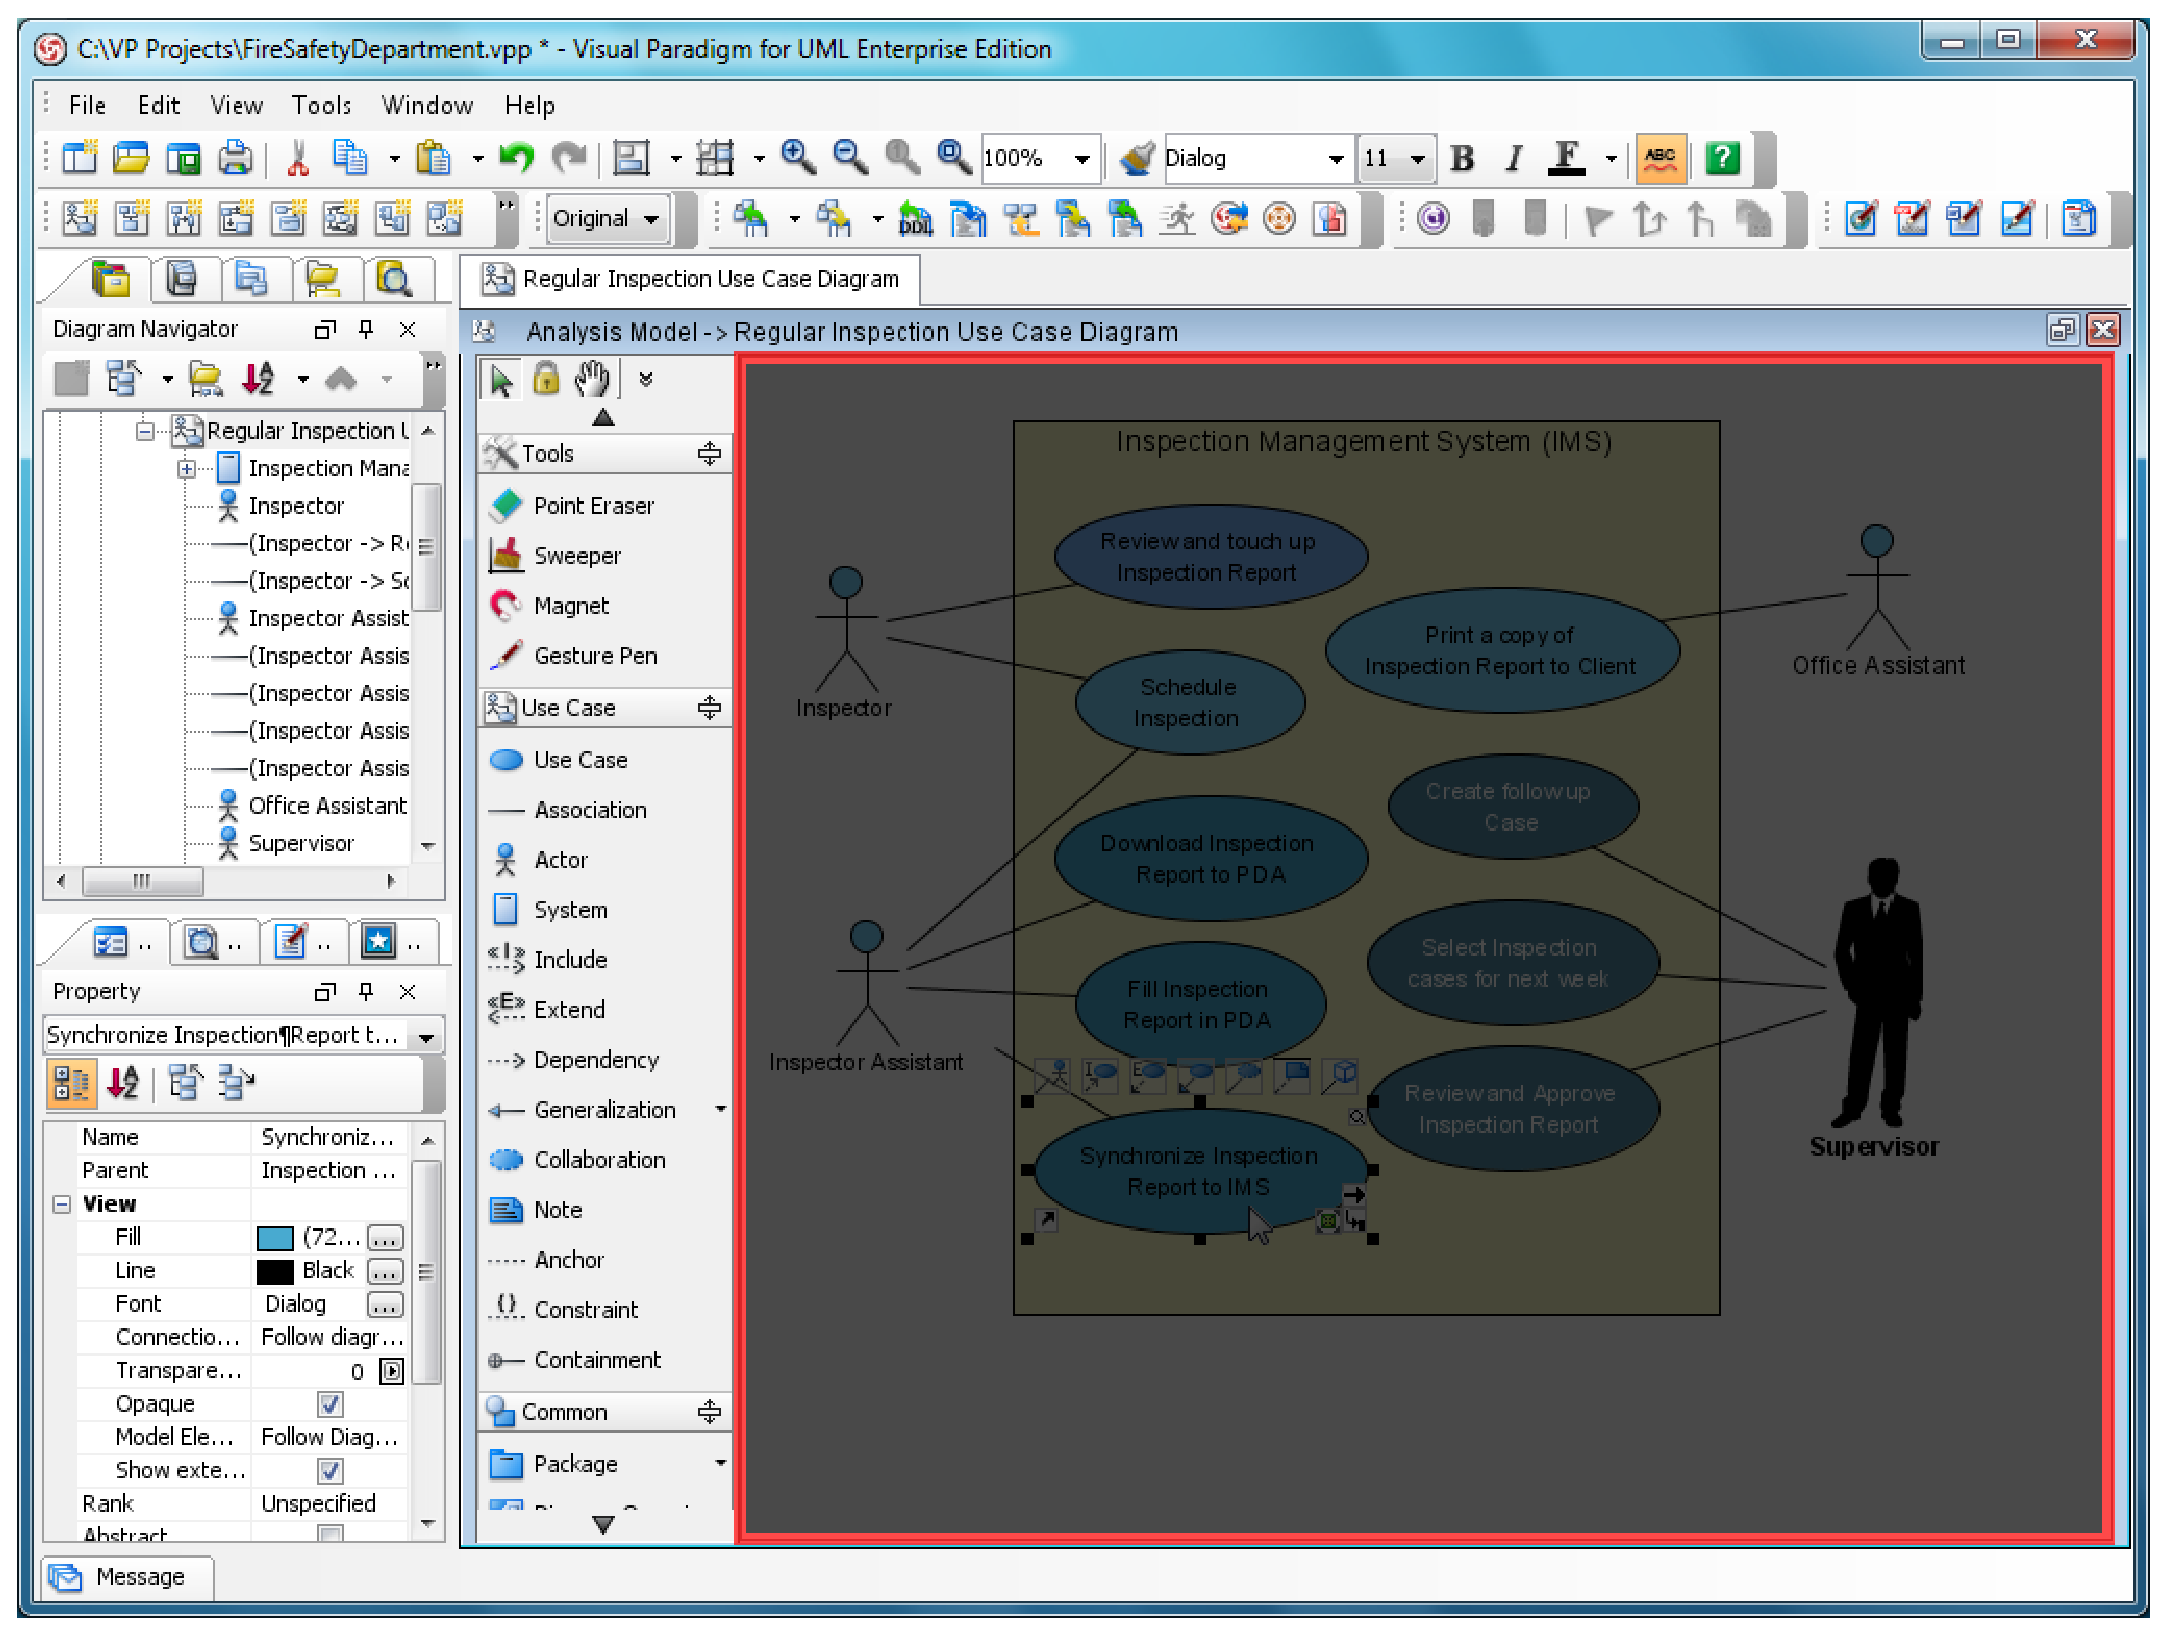
\includegraphics[width=3in]{images/clutter_shot}
\caption{Sample \ac{ide} screenshot provided on Mechanical Turk (Visual
Paradigm)}
\label{fig:clutterexample}
\end{figure}


\subsubsection{Evaluation of Efficiency} \label{subsubsec:efficiency}

The evaluation of both interface and essential efficiency involved the creation of use cases for each \ac{ide} and subsequent evaluation of the corresponding concrete use cases.
We developed two essential use cases common to all \acp{ide} and a third one that differed slightly for each.
The three essential use cases were ordered of increasing task complexity.
\es{Give more detail on the content of the use cases.}
Each essential use case was then manually performed within the \acp{ide} to generate corresponding concrete use cases.
Every physical action required for completion was tracked: keystrokes, mouse clicks, and fine mouse movements.

After all concrete use cases were completed, we noticed that the results from the first two (less complex) use cases did not vary significantly enough across \acp{ide}.
We therefore report only the results from the more complex use case for each \ac{ide}.
